\begin{figure}[h] \centering
	\centering
	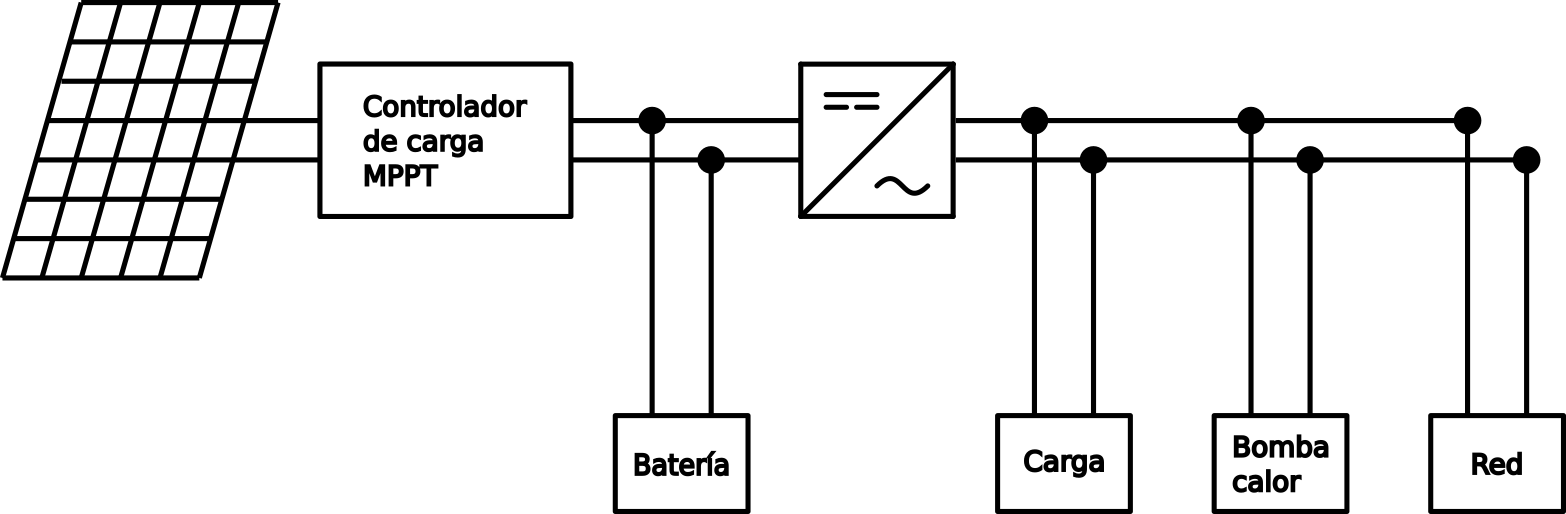
\includegraphics[width=1\textwidth]{./capitulos/resultados_discusion/images/diagrama_electrico.png}
	\caption{Diagrama eléctrico.}
	\label{fig:electic_diagram}
\end{figure}

Tenemos un sistema con paneles fotovoltaicos conectados a un controlador de
carga MPPT (Maximum Power Point Tracking) que con un controlador de electrónica
de potencia regula la tensión de salida de los paneles para obtener el máximo
de potencia en la curva P-V (figura \ref{fig:solar_P-V_I-V}) a través de algún
algoritmo, como el 'Perturb and Observe' (P\&O), donde se actualiza el valor de
la tensión de referencia con el gradiente de la potencia respecto a la tensión.

\begin{equation}
	V_{k} \leftarrow V_k + \alpha \frac{P_k - P_{k-1}}{V_{k}-V_{k-1}}
\end{equation}

\begin{figure}[h] \centering
	\centering
	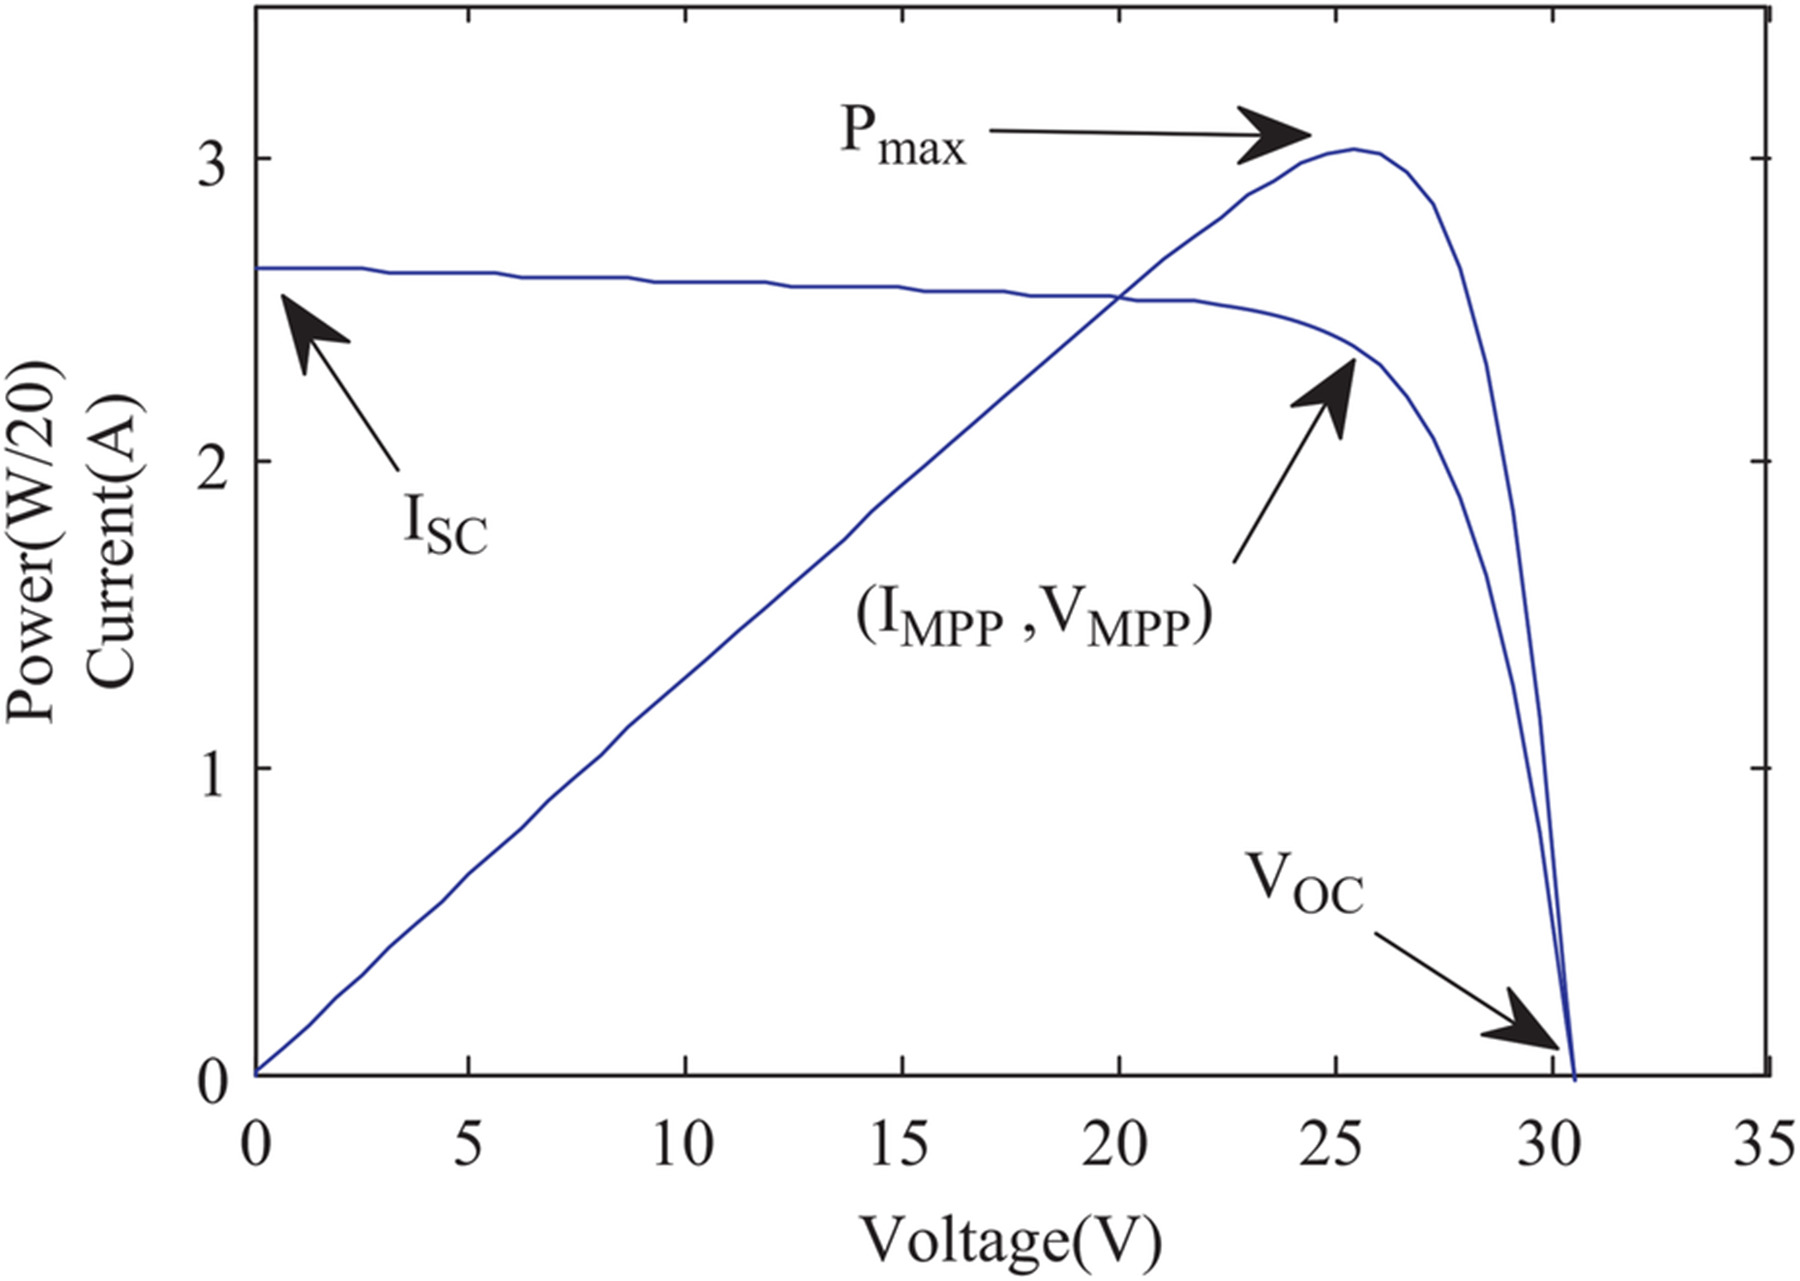
\includegraphics[width=0.6\textwidth]{./capitulos/resultados_discusion/images/solar_P-V_I-V.jpg}
	\caption{Curvas P-V e I-V para un panel solar \cite{podder2019mppt}.}
	\label{fig:solar_P-V_I-V}
\end{figure}


La batería elegida es de tipo LiFePO4 (litio-ferrofosfato) que es comunmente
empleada en aplicaciones de almacenamiento energético. Con tensión nominal total
de 48V.

Conectado al lado de alterna a través de un convertidor DC/AC bidireccional,
donde tenemos la demanda de energía del domicilio (carga), la potencia
destinada a la bomba de calor (compresor), y finalmente está la red, de donde
podemos obtener o volcar energía. Por lo general los precios de compra y venta
son distintos, y así hemos reflejado, usando el precio de mercado diario como
el precio de venta de excedentes, y PVPC (Precio Voluntario para el Pequeño
Consumidor) como el precio de compra, que es mayor que el anterior al incluir
peajes y cargos regulatorios.

En caso de funcionamiento off-grid, reemplazamos la red por un generador diesel
con un precio fijo del combustible, e imponiendo la restricción de que no
podemos volcar energía a este.


Tomando todas las potencias en alterna, el balance energético de esta
instalación queda reflejado por:

\begin{equation}
	P_{red} + P_{solar} = P_{carga} + P_{bat} + P_{bomba}
\end{equation}

donde se han tomado como positivas las potencias de entrada al nodo, y potencia
positiva positiva para la red en caso de demandar energía de esta, y para la
batería cuando se está cargando. Como se refleja en la figura
\ref{fig:electric_node}

\begin{figure}[h] \centering
	\centering
	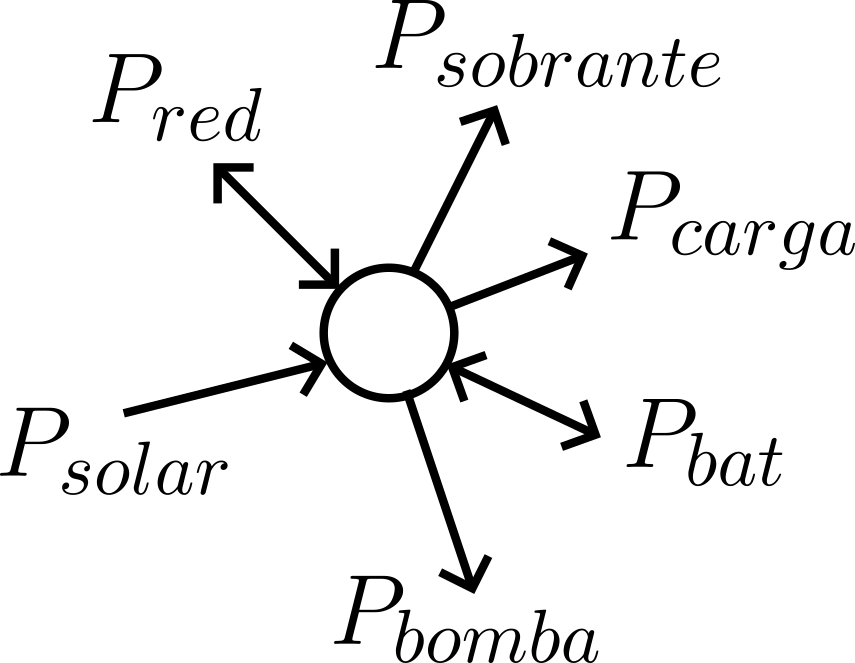
\includegraphics[width=0.4\textwidth]{./capitulos/resultados_discusion/images/electric_node.png}
	\caption{Balance de potencias eléctricas.}
	\label{fig:electric_node}
\end{figure}

La dinámica de las baterías corresponde a

\begin{equation}
	\frac{de}{dt} = \mu_{bat} P_{bat}
\end{equation}

donde $e$ es la energía almacenada, $P_{bat}$ la potencia de alimentación a la
batería y $\mu_{bat}$ la eficiencia de conversión desde alterna a energía
almacenada.

Y a esta le aplicamos las restricciones para los niveles de carga máximo y
mínimo, SOC (State Of Charge)

\begin{equation}
	\text{SOC} = \frac{e}{e_{max}}
\end{equation}

\begin{equation}
	\text{SOC}_{min} \leq \text{SOC} \leq \text{SOC}_{max}
\end{equation}

donde $e_{max}$ es la capacidad, o energía máxima que puede acumular la batería.

Aplicamos como condición inicial que esté en su punto mínimo de carga, partimos
de que está 'vacía'

\begin{equation}
	e_0 = e_{max} \text{SOC}_{min}
\end{equation}

Y la potencia máxima con la que podemos cargar o descargar es función de la capacidad,
a través del factor C-rate, que para células de LiFePO4 establecimos era de aproximadamente
0.3 el valor recomendado, mientras que el máximo nominal de contínuo funcionamiento era de 1.

Podemos relacionar la capacidad y potencia máxima, primero sabiendo que
el C-rate se define como la relación entre la corriente máxima y la capacidad en amperios-hora

\begin{equation}
  i_{max}[A] = \text{C}[Ah] \text{C-rate}
\end{equation}

y luego multiplicando ambos miembros por la tensión nominal

\begin{align}
  i_{max}[A] \, v[V] &= v[V] \, \text{C}[Ah] \, \text{C-rate} \\
  P_{bat_{max}} &= e[Wh] \, \text{C-rate}
\end{align}

Cuando tratemos de sacar las dimensiones optimas de baterías, bomba de calor y
potencia contratada de red, tendremos como variables de diseño la capacidad de
la batería (de donde sacamos la potencia máxima de la batería), y potencía
máxima del compresor y de red respectivamente.

Y estos valores máximos los aplicaremos como restricciones para las variables
de control $P_{bat}$, $P_{red}$ y $P_{bomba}$.

\begin{align}
  -P_{bat_{max}} < P_{bat} < P_{bat_{max}} \\
  -P_{red_{max}} < P_{red} < P_{red_{max}} \\
  0 < P_{bomba} < P_{bomba_{max}}
\end{align}
